\documentclass[
    11pt,
    spanish,
	a4paper
]{article}
\usepackage[utf8]{inputenc}
\usepackage[spanish]{babel}
\usepackage{graphicx}
\usepackage{authoraftertitle}
\usepackage{float}
\usepackage{caption}
\captionsetup[table]{labelformat=empty}

\def\doctype{TRABAJO PRÁCTICO FINAL}
\title{Unidad Aritmética lógica}
\author{Gonzalo Nahuel Vaca}

\begin{document}

\makeatletter
\begin{titlepage}
	\begin{center}
		\vspace*{1cm}
		
		\Huge
		\textbf{\doctype}
		
		\vspace{0.5cm}
		\LARGE
		\@title
		
		\vspace{1.5cm}
		
		\textbf{\@author}

		\vspace{3.5cm}

		
\includegraphics[width=0.8\textwidth]{img/logoFIUBA.pdf}
		
		\vfill
		Facultad de Ingeniería\\
		Universidad de Buenos Aires\\
		Argentina\\
		\today
	\end{center}
\end{titlepage}
\makeatother
\newpage

\section{Introducción}
\label{sec:introduccion}

\subsection{Propósito}
\label{subsec:proposito}

Este trabajo tiene como propósito detallar el desarrollo de una \emph{Unidad Aritmética Lógica}.

\subsection{Alcance}
\label{subsec:alcance}

El trabajo fue realizado en el marco de la materia \emph{Circuitos Lógicos Programables} y consta de las siguientes etapas:

\begin{itemize}
    \item Creación de un archivo de \emph{register transfer level} en \emph{vhdl}.
    \item Creación de un archivo de simulación y estímulo en \emph{vhdl}.
    \item Síntesis e implementación para un kit \emph{ARTYZ720}.
    \item Creación de un archivo de \emph{bitstream}.
    \item Montaje de placa de entradas.
\end{itemize}

\section{Descripción general}
\label{sec:descripcion}

\subsection{Introducción general}
\label{subsec:teorica}

Una Unidad Aritmética Lógica (ALU) es un circuito digital que realiza operaciones aritméticas (suma, resta) y operaciones lógicas (and, or, xor).
Las operaciones se realizan sobre uno o dos operandos.
En la figura \ref{fig:ejemplo} se puede observar un ejemplo de representación de una ALU.

\begin{figure}[h!]
    \centering
    
\includegraphics[width=0.4\textwidth]{img/alu_example.png}
    \caption{Ejemplo de una ALU.}
    \label{fig:ejemplo}
\end{figure}

\subsection{Register Transfer Level}
\label{subsec:rtl}

En esta etapa se realizó la descripción del funcionamiento de la ALU para su posterior proceso de sintetizado.
En la figura \ref{fig:rtl_sim} se puede observar una simulación del código generado mientras que en la figura \ref{fig:rtl_sch} se puede ver el diagrama en bloques que representa la funcionalidad.

\begin{figure}[h!]
    \centering
    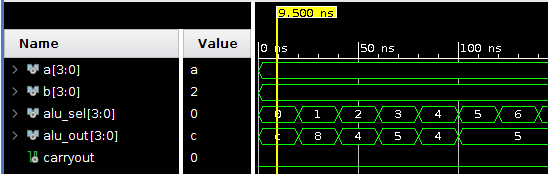
\includegraphics[width=0.8\textwidth]{img/rtl_sim.png}
    \caption{Simulación rtl.}
    \label{fig:rtl_sim}
\end{figure}

\begin{figure}
    \centering
    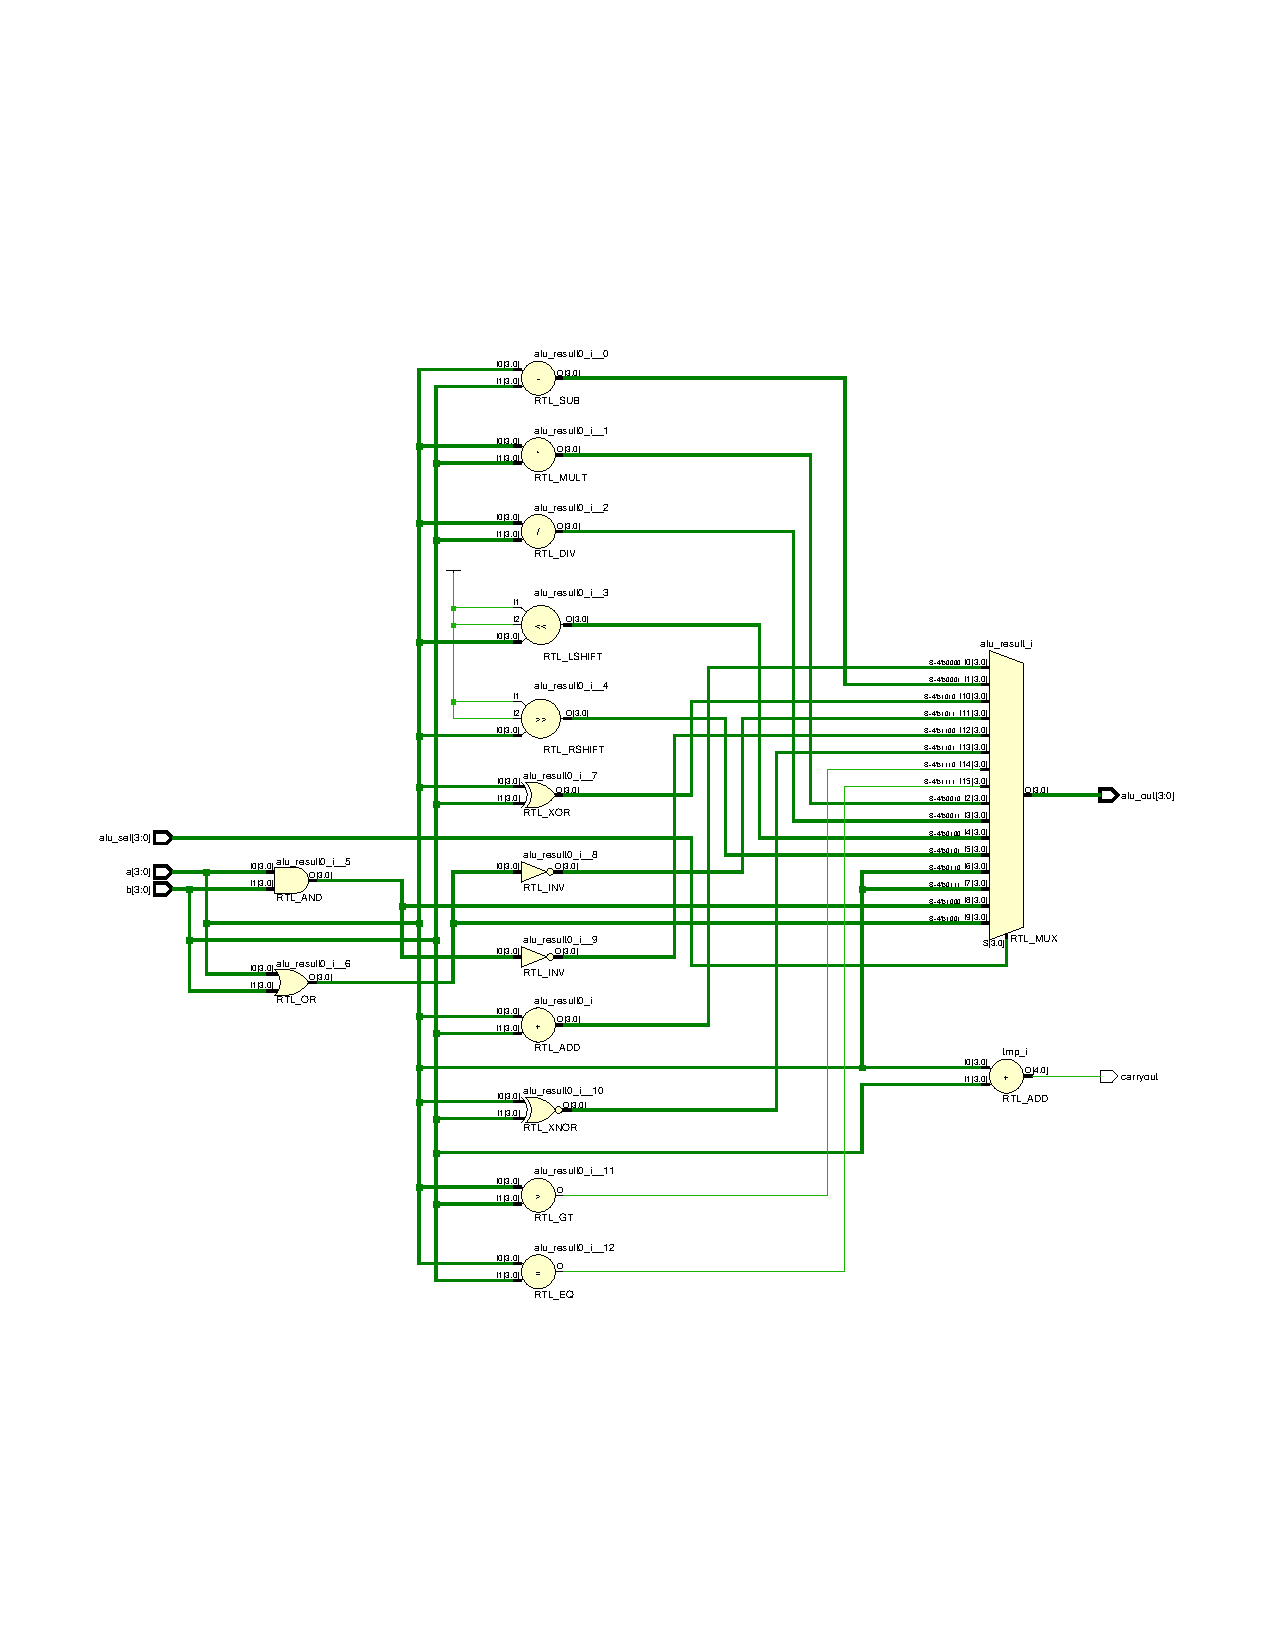
\includegraphics[width=\textwidth]{img/rtl_schematic.pdf}
    \caption{Esquemático rtl.}
    \label{fig:rtl_sch}
\end{figure}

\subsection{Síntesis}
\label{subsec:sintesis}

En esta etapa se determina si el comportamiento descripto es realizable.
En el caso de este proyecto el esquemático del modelo sintetizado se puede observar en la figura \ref{fig:syn_sch}.

\begin{figure}
    \centering
    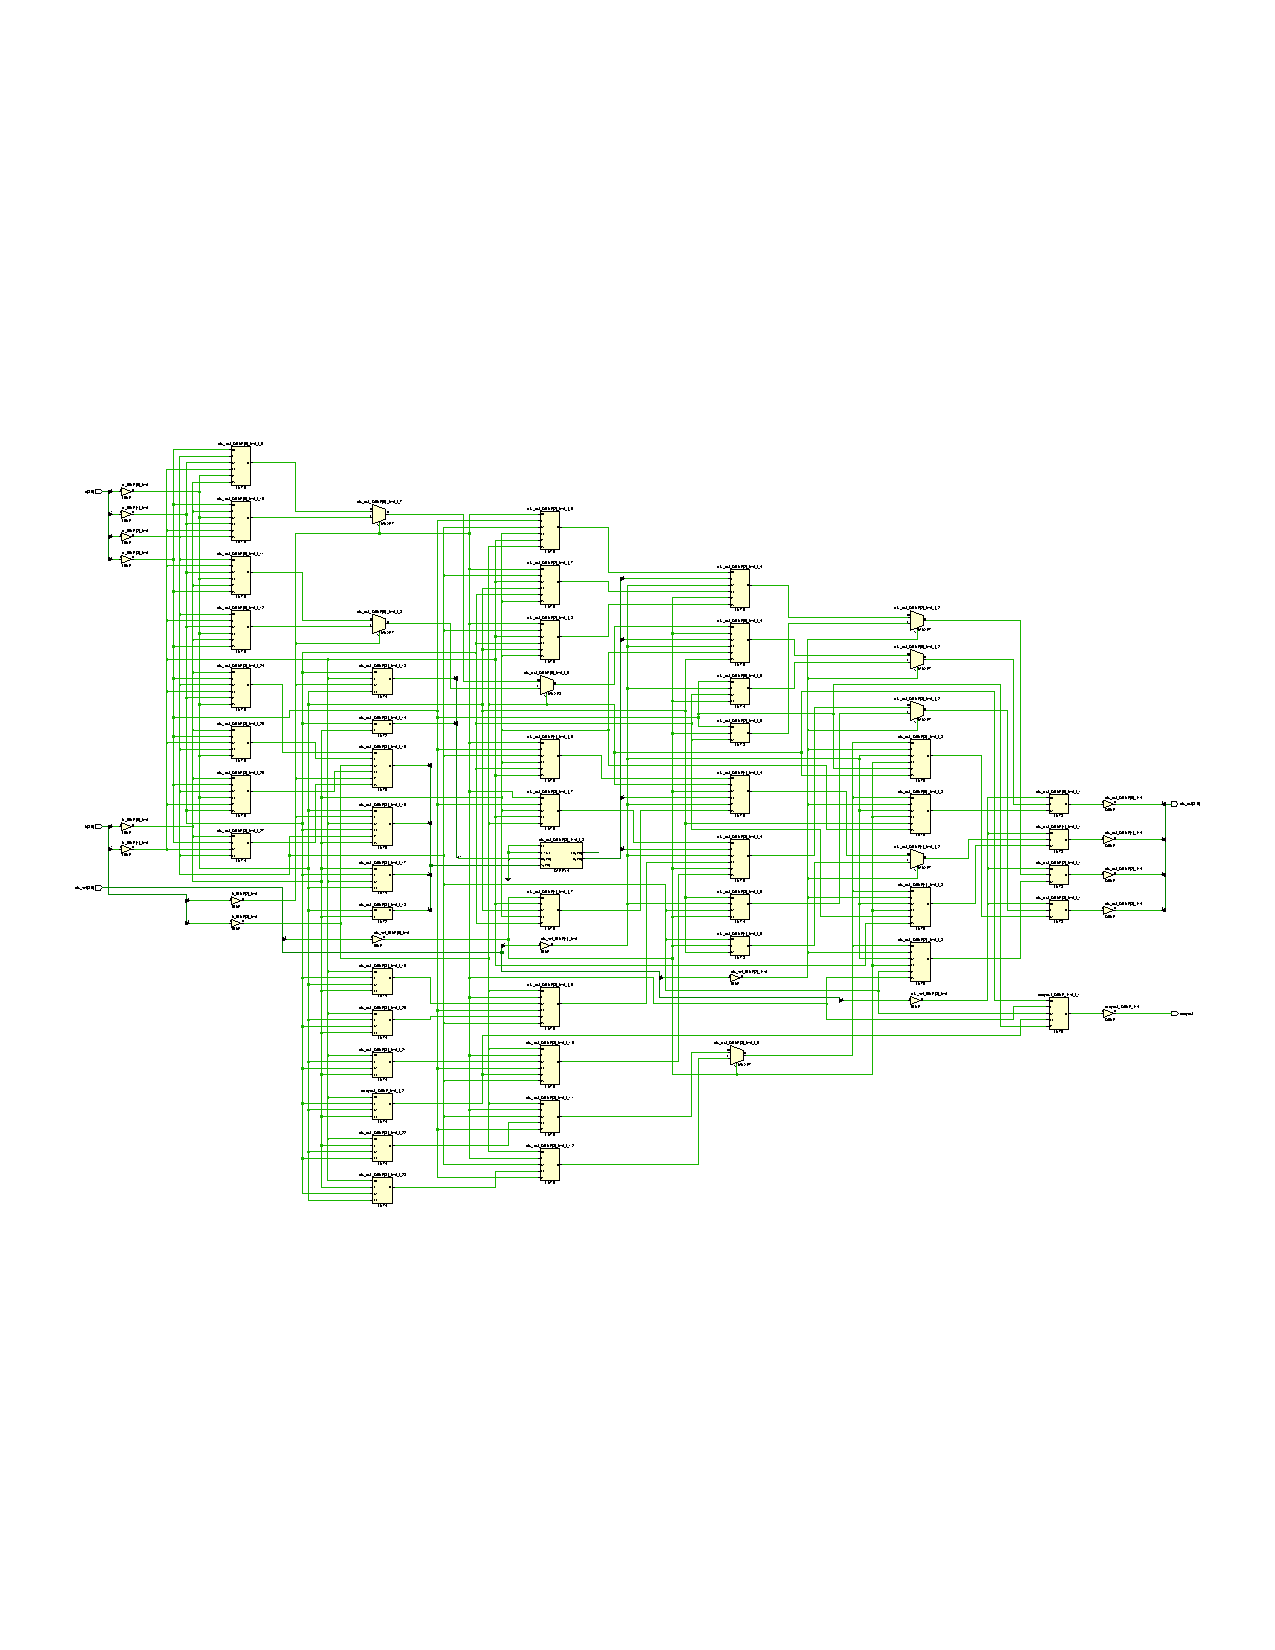
\includegraphics[width=\textwidth]{img/syn_schematic.pdf}
    \caption{Esquemático de la síntesis.}
    \label{fig:syn_sch}
\end{figure}

\subsection{Implementación}
\label{subsec:implementación}

En esta etapa se asignan los recursos de la \emph{FPGA}.
En la figuras \ref{fig:imp_table} \ref{fig:imp_device} se pueden observar como \emph{Vivado} asignó los recursos dentro del integrado.

\begin{figure}[h!]
    \centering
    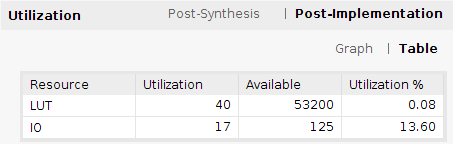
\includegraphics[width=0.8\textwidth]{img/imp_table.png}
    \caption{Tabla de recursos.}
    \label{fig:imp_table}
\end{figure}

\begin{figure}
    \centering
    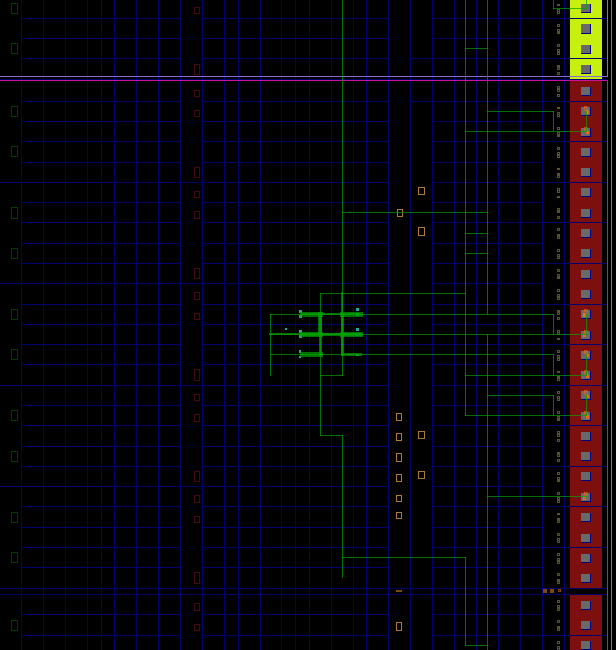
\includegraphics[width=\textwidth]{img/imp_device.png}
    \caption{Asignación de recursos en la \emph{FPGA}.}
    \label{fig:imp_device}
\end{figure}

\subsection{Bitstream}
\label{subsec:bitstream}

El paso final dentro del entorno de \emph{Vivado} fue crear las instrucciones a transmitir para que realicen las conexiones internas dentro la \emph{FPGA}.
Luego, se procedió a volcar el \emph{bitstream} dentro del integrado.

\subsection{Montaje}
\label{subsec:montaje}

En la figura \ref{fig:montaje} se puede observar el resultado final del proyecto.

\begin{figure}
    \centering
    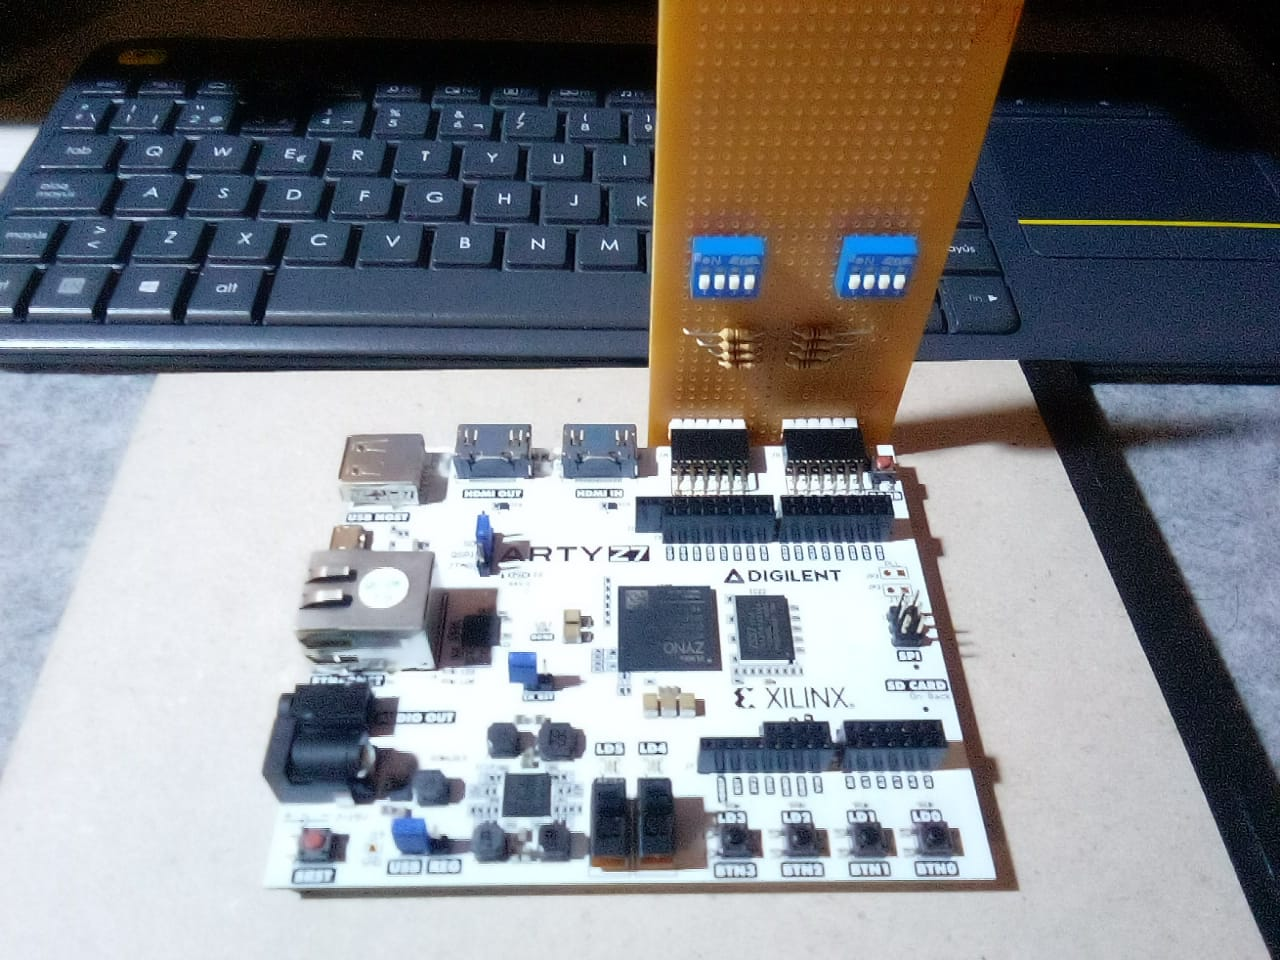
\includegraphics[width=\textwidth]{img/montaje.jpeg}
    \caption{Montaje.}
    \label{fig:montaje}
\end{figure}

\end{document}
